\documentclass[12pt,psfig,a4]{article}
\usepackage{geometry}
%\geometry{a4paper}
\geometry{left=28mm,right=28mm,top=21mm,bottom=21mm}

%\gemoetry{verbose,a4paper,tmargin=21mm,bmargin=21mm,lmargin=18mm,rmargin=18mm}
\usepackage{graphics}
\usepackage{setspace}
\usepackage{url}
\usepackage{listings}
\newcommand{\Lyx}{L\kern-.1667em\lower.25em\hbox{y}\kern-.125emX\spacefactor1000}
\newcommand\bibname{References}
\singlespacing
%\setlength{\parskip}{0pt}
%\setlength{\parsep}{0pt}
%\setlength{\headsep}{0pt}
%\setlength{\topskip}{0pt}
%\setlength{\topmargin}{0pt}
%\setlength{\topsep}{0pt}
%\setlength{\partopsep}{0pt}
\usepackage[compact]{titlesec}
\titlespacing{\section}{0pt}{*1}{*1}
\titlespacing{\subsection}{0pt}{*1}{*1}
\titlespacing{\subsubsection}{0pt}{*1}{*1}

\begin{document}
\bibliographystyle{plain} 
\pagestyle{plain} 
\pagenumbering{arabic}
%\rmfamily
\newenvironment{code}
{\sffamily
 \setlength{\parskip}{0pt}
}
{}

\title{\vspace{2in}\textbf{
COMS W4115 Fall 2011\\
Course Project\\
TML Final Report}}
\author{
Jiabin Hu (jh3240)\\
Akash Sharma (as4122)\\
Shuai Sun (ss4088)\\
Yan Zou (yz2437)\\\\
\textit{Columbia University}
}
\date{\textit{December 21th, 2011}}
\maketitle

\pagebreak
\tableofcontents


%Akash Begin
\pagebreak
\section{Introduction}

\subsection{Motivation}
Tree is one of the most fundamental data structures not only in computer science, but also in real life. The applications built on it range from data storing and searching to coding and routing algorithms. However, in most modern programming languages, representing a tree requires pointers or references, which often leads to bugs that are hard to catch. Furthermore, codes on tree manipulation are usually difficult to read, since they hardly reflect the abstracted operation. Therefore, we plan to design a new language, the Tree Manipulating Language (TML), specifically for manipulations on trees. The goal of the language is to provide more efficient and user-friendly programming methods to implement operations on trees.

\subsection{Overview}
Tree manipulation language (TML) is a user friendly language that is designed to help users program trees. It allows users to create, manipulate and run algorithms on trees. Various existing programming languages make tree operations cumbersome and TML is intended to bridge this gap. In TML everything is of type Tree except primitive data types. Each node of the tree is of type Tree and it has fields associated with it like parent, child etc. Every node of the Tree is root for its subtree. Nodes of the tree can consist of user defined or primitive value types and they can be of any degree. We can refer to any child or parent node of a given node using predefined constructs. TML provides methods to perform trivial operations on trees such as tree traversal, node creation or deletion etc.

In TML, we introduce a new type named type \textbf{\emph{Tree}}. As our language is specifically designed for tree programs, incurring a type \textbf{\emph{Tree}} will make it easier to program. Basic operations to program on a tree are provided in our language, such as tree construction, adding tree node, referring to father, referring to root data, etc. Programmers could both use the provided operation or define new functions to manipulate trees.

\begin{figure}[hb]
{\centering \resizebox*{250pt}{150pt}{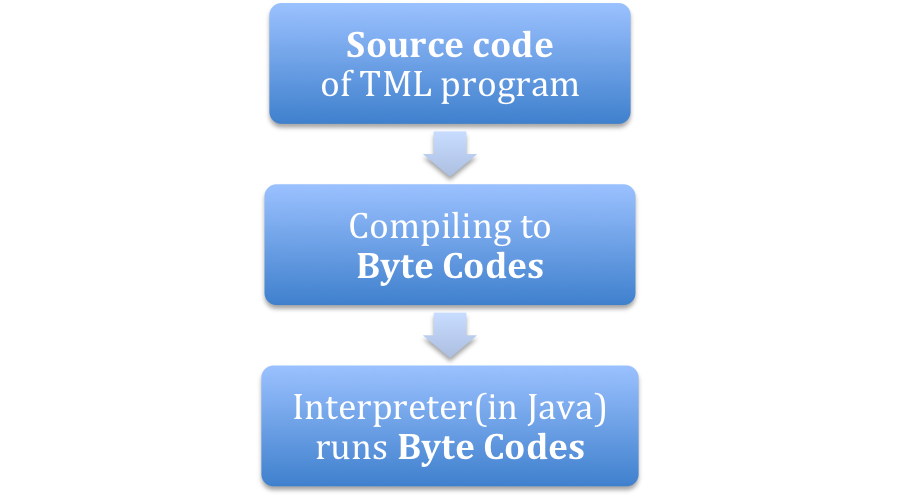
\includegraphics{Process.png}} \par}
\caption{TML Compiling Process}
\label{TCP}
\end{figure}

The main concept of our language is that, everything except primitive types is regarded as a tree, just like everything in Java is an object. Noted that every child of a tree is the root of its sub-tree. In TML, we regard all nodes in a tree as sub trees which are of the same type as the original one. When applying operations on a tree, we recursively apply the operations on sub trees and the root. The recursive feature of trees is the reason for this language feature. For operations on a single node, reference to the node is available by referring to its sub tree.

In TML, users can define new types of tree inherited from the basic type \textbf{\emph{Tree}}. The degree and storage field can also be user-defined. Users could use this feature to build their own trees and even queues, stacks, lists, etc.

TML compiles the source codes and translate them into TML byte code, which is then interpreted by TML interpreter to execute the program. The compiler and byte code generator is implemented in OCaml, and the interpreter is written in Java Figure \ref{TCP} shows the translation process of TML.

\pagebreak
\section{Language Tutorial}
TML was designed to describe trees and use them in a more convenient way, with language-supported tree operators. User of TML can use these feartures to define their own tree-like data structures and write their programs.

\subsection{An Introduction}
TML is a C-like language. Most of the grammer is similar to that of C. Each source file, with the extension ".tml", should contain a main() method, which returns nothing. And each statement in the code should end with a semicolon.

\begin{code}
\begin{tabbing}
~~~~~~~~\= void \=main () \\
\> \{ \\
\> \> // tml statements.\\
\> \}
\end{tabbing}
\end{code}

TML includes primitive types, which are integer, float, character, boolean, and string. These types are used in the way just like in C and C++, only that in TML, no type conversion is allowed. Also, user can define their own types of tree in TML. The definition of the tree type should appear before they are used in other parts of the program. Below is an example of user defined binary tree.

\begin{code}
\begin{tabbing}
~~~~~~~~\= treet\=ype \textless2, [left, right]\textgreater MyTree\_t \\
\> \{ \\
\> \>int vint = 0;\\
\> \>float vflt = 1.;\\
\> \>string vstr = ''hi '';\\
\> \}
\end{tabbing}
\end{code}

User can declare new instances of tree types in the same way in C. To allocate memory space of an instance, user can use the built-in alloc function.
TML programs can output results of computation by using built-in printing function.

\begin{code}
\begin{tabbing}
~~~~~~~~\=MyTree\_t ta;~~~~~~~// declare new instance\\
\> alloc (ta);~~~~~~~~~~// alloc memory\\
\> ta.vint = 15;\\
\> print (ta.vint);~~~~// prints out 15.\\
\end{tabbing}
\end{code}

When your finish writing the code, to compile the program, type the following command line:
\begin{code}
\begin{tabbing}
~~~~~~~~\=./tmlc sample\_program.tml\\
\> ./tml\\
\end{tabbing}
\end{code}

\subsection {An Example of Tree Traversal}
The following code of TML is an example of inorder traversal over the tree. In the program, it defineds a binary tree type, constructs a tree with tree operators, sets the value and prints the result.
The tree constructed along with the value set is in the figure~\ref{bintree}.

\begin{figure}[h!]
{\centering \resizebox*{100pt}{86pt}{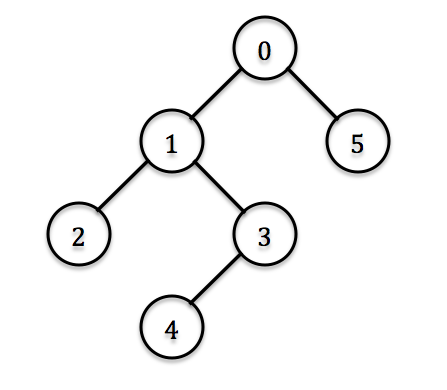
\includegraphics{tree.png}} \par}
\caption{Tree constrution in sample code}
\label{bintree}
\end{figure}

\begin{code}
\begin{tabbing}
~~~~~~~~\= treet\=ype \textless2, [left, right]\textgreater MyTree\_t \\
\> \{ \\
\> \>int val = 0;\\
\> \}\\
\>  void main () \\
\> \{ \\
\> \> int i = 0;\\
\> \> MyTree\_t a, b, c, d, e, f;\\
\> \> alloc(a, b, c, d, e, f);\\
\> \> a -\textgreater ( b -\textgreater ( d : e -\textgreater ( f : $\sim$ ) ) : c);\\
\> \> foreach node in a by preorder\\
\> \> \{\\
\> \> ~~~~node.val = i;\\
\> \> ~~~~i = i + 1;\\
\> \> \}\\
\> \> foreach node in a by inorder\\
\> \> \{\\
\> \> ~~~~print(node.val);\\
\> \> ~~~~print(`` ");~~~~~~~~// print a space\\
\> \> \}\\
\> \}
\end{tabbing}
\end{code}

Now, you have already written a program in TML. You can compile it and run. It should prints out:
\begin{code}
\begin{tabbing}
~~~~~~~~2~1~4~3~0~5\\
\end{tabbing}
\end{code}


\pagebreak
\section{Language Manual}

\subsection{Lexical Conventions} \label{lexCon}
There are different classes of tokens that are supported in TML. Token types are identifiers, keywords, literals, strings and operators. As in C language, whitespace characters are ignored except insofar as they serve to delineate other tokens in the input stream. If the input stream has been parsed into tokens up to a given character,the next token is taken to include the longest string of characters which could possibly constitute a token.

%Akash: try to reorganize the sentences

\subsubsection{Character Set}
TML takes the standard \textbf{ASCII} character set for source codes.

\subsubsection{Comments}
In TML, there are two ways to make comments. The first style starts with the characters \textbf{/*}, and ends with the characters \textbf{*/}, all contents between which are comments. Note that, just like C-style comments, TML supports only un-nested comments. The second style is inline comments. It starts with the characters \textbf{//}, all contents in the current line after which are regarded as comments.

\begin{code}
\begin{tabbing}
~~~~~~~~\= /*  \=\textit{This is a} \\
\> \> \textit{block comment.} */\\
\> // \textit{This is an inline comment}.
\end{tabbing}
\end{code}

\subsubsection{Identifiers} \label{lexConId}
In TML, an identifier is a string that starts with a letter or an underscore, and consists of a sequece of letters, digits, and underscores. %The max length of an identifier is 26 characters. 
All identifiers are case-sensitive in TML.

\subsubsection{Keywords}
%\textit{This section needs discussion.}\\
In TML, the words listed in Table~\ref{keywords} are reserved as keywords, and are not allowed to be used as a user-defined identifier.

\begin{table}[!ht]
\begin{center}
\begin{tabular}{| c | c | c | c | c |}
\hline
if & else & do & while & for \\
\hline
break & continue & foreach & in & by     \\  %%whether remove the keyword do??         %Shuai: yes, keep it for do-while-loop
\hline
return & void & main & print & alloc \\
\hline
preorder & inorder & postorder & levelorder & treetype\\
\hline
int & float & char & string & bool \\
\hline
true & false & & &\\
\hline
\end{tabular}
\caption{Keywords in TML}
\label{keywords}
\end {center}
\end{table}
%Akash End

% Shuai Begin
\subsubsection {Constants}
There are several kinds of constants in TML, which are listed as follows.

\begin{itemize}
\item Integer constants
An integer constant consists of a sequence of digits, starting with a non-zero digit. All integer constants are considered to be decimal and of type integer.

\item Float constants
A floating constant consists of an integer part, a decimal point, a fraction part, and optionally an `e' with a signed integer exponent. The integer and fraction parts both consist of a sequence of digits, and either one could be missing, but not both. Either the decimal point or the `e' with the exponent could be missing, but not both. All floating constants are of type float.

\item Character constants
A character constant is a single ASCII character enclosed by $'$ $'$, which is of character type. Note that $'$\textbackslash$n'$, $'$\textbackslash$t'$, and $'$\textbackslash$r'$, are character constants.

\item String constants
A string constant consists of several character constants enclosed by $''$~~~$''$, and implicitly ends with $'$\textbackslash$0'$.

\item Boolean constants
There are only two boolean constants, \textit{true} and \textit{false}.

\item Tree constant
There is only one tree constant, which is the null constant. The null constant is a null value of any tree type. If a tree is null, then it means the tree reference is lost at the point of time. In TML, the null constant is written as a tilde, `$\sim$'.

\end{itemize}

\subsection {Types}
In TML, there are two kind of types, the \textit{primitive types} and the \textit{tree types}.

\subsubsection {Primitive Types}
There are several kinds of primitive types. The size and value range of each type is listed in Table~\ref{pri_types}. The type specifiers can be found in section~\ref{typeSpec}

\begin{table}[!ht]
\begin{center}
\begin{tabular}{| c | c | c | c |}
\hline
\textbf{Primitive Type} & \textbf{Size} & \textbf{Range} & \textbf{Default value} \\
\hline
Integer & 4 bytes & -2 147 483 648 ~  2 147 483 647 & 0 \\
\hline
Float & 4 bytes & about $\pm$3.402 823 47E+38 & 0.0\\
\hline
Character & 2 byte &  ASCII & $'$\textbackslash$0'$\\  % check the java and boolean
\hline
String & $\geq$ 1 byte & combinations of characters & $'$$'$$'$$'$\textit{(empty)} \\
\hline
Boolean & 4 bytes & true, false & false \\
\hline
\end{tabular}
\caption{Primitive Types in TML}
\label{pri_types}
\end {center}
\end{table}


\begin{itemize}
\item Intergers
In TML, there is only one type of integer. The integers are signed, and are of fixed size. The size of an integer is four bytes.

\item Floating point numbers
In TML, there is only one type of floating point number. The size of the float type is four bytes.

\item Characters
In TML, there is only one type of character. The size of a character is two bytes. The characters are interpreted as ASCII code.

\item Strings
Strings are considered as a primitive type in TML. A string is a permutation of more than one characters. A string can be compared with another string. The size of a string equals to the number of characters in it.

\item Booleans
Boolean type is a primitive type in TML. There are only two values, true and false, in the Boolean type, which is used to determinate logic conditions. There is no conversions between integers and these two values.

\end{itemize}

\subsubsection {Tree Types}
In TML, a \textit{tree type} is a type to represent trees. By using the tree types, users can define and use tree data structures in their programs.

In a tree data structure, children of the root node can be also regarded as roots of sub trees. By this concept, in TML, all nodes in a tree are of the same tree type with the root. There is no tree node type in TML.

\begin{itemize}
\item Define a tree type
\label{defTreetype}
Tree types are defined by users before they can declare and define variables of the tree types. A tree type consists of necessary parts, \textit{type name}, \textit{degree} and \textit{member variable(s)}, and an optional part, \textit{children index aliases}. To define a tree type, the \textit{type name}, \textit{degree} and \textit{member variable(s)} must be defined, and the \textit{children index aliases} can be optionally defiined. The size of a tree type is the sum size of its member variable types.

When defining each member variable, an intial value can be optimally defined. If the initial value of a member variable is not defined, it will be intialized with the default value of each type. For primitive types, the default values are defined in Table~\ref{pri_types}. For tree types, it will be assigned with null.

An example of a tree type definition, MyTree\_t, is given below.

\begin{code}
\begin{tabbing}
~~~~~~~~\= treet\=ype \textless2, [left, right]\textgreater MyTree\_t \\
\> \{ \\
\> \>int vint = 0;\\
\> \>float vflt = 1.;\\
\> \>string vstr = ''hi '';\\
\> \}
\end{tabbing}
\end{code}

\item Type name
The \textit{type name} of a tree type follows the identifier definition in the section~\ref{lexConId}. After the tree type is defined, the type name can be used to define variables of this type.

\item Degree
In TML, each tree type must define a fixed \textit{degree} at definition. All nodes of the same tree type have the same degree. The value range of the degree is from 1 to 99. The degree of a tree type can be referred to by using  the operator ``\&'' introduced in the section~\ref{treeOp}.

% use &a  to get the degree

\item Member variables
In TML, a tree type can define its own \textit{member variable(s)} to store values for algorithms and programs. Each tree type can have at most 99 member variables. Each member variable must have a name which is unique in its tree type, and can be of any primitive types or tree types. Note that if a member variable is defined as some tree type, the definition of the tree type must appear before the member variable definition. All member variables are public. The member variables of a tree type variable can be referred to by using dot operator introduced in the section~\ref{treeOp}.

% limit the member tree varible have only primitive types

\item Children index and aliases
In TML, children sub roots of a root can be referred to by the index number, ranging from 0 to (degree-1). Optionally, at the definition of a tree type, user can define alias of the children indices. The alias follows the identifier definition in section~\ref{lexConId}. Note that if aliases are defined, then aliases for all Children indices must be defined. Only defining a subset of children indices is not allowed in TML. Whether using number indices or aliases, the children of a tree root can be referred to by using child access operator introduced in section~\ref{treeOp}.

\end{itemize}

\subsubsection {Type Conversions}
In TML, no type conversion is allowed.

% Shuai End

% Jiabin Begin

\subsection{Expressions}
In TML, expressions consist of operators and their operands. In this section, definition for each operator is given. To avoid ambiguity, precedence rules of the operators in TML are also defined in this section.

\subsubsection{Arithmetic operators}
In TML, arithmetic operators are $+$, $-$, $*$, $/$ and $\%$. $+$ means addition, $-$ means substruction, $*$ means multiplication, $/$ means division and $\%$ means modulation. All of them are binary and left associative. It requires that their operands must be of the same primitive types, and the result will be of the same type.

\subsubsection{Comparative operators}
In TML, comparative operators are $>$ (greater than), $<$ (less than), $>=$ (greater than or equal to), $<=$ (less than or equal to), $!=$ (not equal) and $==$ (equal). All of them are binary operators and left-associative. It requires that their operands must be of the same primitive types . The return value is a boolean value indicates the predicate.

\subsubsection{Logical operators}
Logical operators in TML include $\&\&$ (logical and), $||$ (logical or) and ! (logical not). \&\& and $||$ are binary operators and left-associative. They take two operands of type boolean, and return a boolean value. ! is unary and appears on the left side of the operand. They type of the operand must be of type boolean and the return type is also a boolean value.

\subsubsection{Assignment operators}
TML's assignment operator is =. it's binary operator and right-associative. The left operand must be a legal left value, and the right operand must be an expression. In TML, a legal left value can be a variable, a member variable of a tree type or a child of a tree. When an assignment is taken, the value of the expression on the right is assigned to the left value, and the new value of the left value is returned, which allows chained assignments. 

\subsubsection{Parentheses}
In TML, parentheses in expressions are used to overwrite the precedence rules. Expression enclosed by the parentheses is calculated before applying its adjacent operators.

\subsubsection{Tree Operators}
The TML is a set of operators that can be applied to trees. They are divided into three categories: tree-building operators, tree-copying operators and tree-querying operators.

\begin{itemize}
\item Tree-building operators
The operator -\textgreater is the tree building operator. This operator is used to connect the root and its children to build a tree. It is binary and right-associative. Its left operand is a single tree node, representing the root. The right operand is a list of children trees, enclosed by parentheses. Each child tree is separated by colons, representing the immediate children of the root. An example is given below. In this example, a tree is built with ta as root and tb as its left subtree, and tc as its right subtree. This operator returns the newly built tree, which is ta.
\begin{code}
\begin{tabbing}
~~~~~~~~\= MyTree\_t ta, tb, tc;\\
\> alloc(ta, tb, tc);\\
\> ta~-\textgreater(tb : tc);
\end{tabbing}
\end{code}

\item Tree-copying operators
In TML, two operators are supplied to copying trees. They are the At(@) operator and the Dollar(\$) operator. Both of them are right-associative. And they both take only one operand of a tree type. 

The At operator copies the root node of the operand and its values only, with all of its children set to null. The Dollar operator copies the whole tree referenced by the operand, including all sub trees and children. Both of them return the reference of the newly-copied tree.

In the example below, ta\_copy1 gets only the ta node with both children set null, while ta\_copy2 get the copy of the whole ta tree, with the two children connected.
\begin{code}
\begin{tabbing}
~~~~~~~~\= MyTree\_t ta, tb, tc;~~~~~~~\=\\
\> alloc(ta, tb, tc);\\
\> ta~-\textgreater(tb : tc);\\
\> MyTree\_t ta\_copy1, ta\_copy2;\\
\> ta\_copy1 = @ta;\>//\textit{copy ta node only}\\
\> ta\_copy2 = \$ta;\>//\textit{copy the whole ta tree }
\end{tabbing}
\end{code}


\item Tree-querying operators
\label{treeOp}
In TML, several tree-querying operators are defined to get properties of a tree. They are the \textbf{Hash(\#)} operator, the \textbf{square bracket operator([])}, the \textbf{Dot(.)} operator, the \textbf{Ampersand(\&)} operator and the \textbf{Caret(\^{})} operator. The detailed definition for each operator is given below, followed by an example to illustrate their usages.

The \textbf{Hash} operator takes one operand of a tree type, and returns and integer representing the order of the operand among its siblings. If the operand has no parent, the return value is -1. 

The \textbf{square bracket operator} is used to get access to children of a tree. It takes two operands, the first on the left of the brackets and the second in the brackets. The first operand is of a tree type, and the second is either an integer index or children alias string index defined at the tree type definition. The return value is the reference to a the required child. Note that the operand inside the square bracket must be less than the degree of the tree. The behavior of an index exceeds the degree of the tree is unknown.

The \textbf{Dot} operator is used to access the data fields associated with the node. It is a binary and left-associative operator. The left operand is of a tree type, and the right operand is the name of a data fields defined at the type definition. The return value is the value of that particular field.

The \textbf{Ampersand} is used to get the degree of tree. It is a unary operator and appears in front of its operand, which is of a tree type. It returns an integer indicating the degree of the tree.

The \textbf{Caret} operator is used to get the parent reference of the operand. It is a unary operator and appears on the left side of the operand, which is of a tree type. It returns the reference of the operand's parent.


\begin{code}
\begin{tabbing}
~~~~~~~~\= MyTree\_t ta, tb, tc;~~~~~~~~~~~~~~~~\=//\textit{MyTree\_t is defined in section~\ref{defTreetype}}\\
\> alloc(ta, tb, tc);\\
\> ta~-\textgreater(tb : tc);\\
\> int ta\_order = \#ta;\>//\textit{ta\_order = -1}\\
\> int tb\_order = \#tb;\>//\textit{tb\_order = 0}\\
\> int tc\_order = \#ta[1];\>//\textit{tc\_order = 1}\\
\> MyTree\_t tb\_copy = ta[0];\>//\textit{tb\_copy has the same ref with tb}\\
\> MyTree\_t tc\_copy = ta[1];\>//\textit{tc\_copy has the same ref with tc}\\
\> MyTree\_t t\_err = ta[2];\>//\textit{this usage could cause unknown errors}\\
\> int tmp1 = ta.vint;\>//\textit{tmp1 has the value of ta.vint, which is 0}\\
\> float tmp2 = tb\_copy.vflt;\>//\textit{tmp2 has the value of tb.vflt, which is 1.0}\\
\> string tmp3 = tc.vstr;\>//\textit{tmp3 is ''hi ''}\\
\> int degree = \&ta;\>//\textit{degree is assigned with 2}\\
\> MyTree\_t ta\_copy = \^{}tb;\>//\textit{ta\_copy has the same ref with ta}
\end{tabbing}
\end{code}

\end{itemize}


\subsubsection{Precedence Rules}
To eliminate the possibility of ambiguity, the precedence of operators in TML are defined in Table~\ref{preRule}.

\begin{table}[ht]
\begin{center}
\begin{tabular}{| c | c |}
\hline
1 & () \\
2 & . ~ , ~ [] \\
2 & \# ~ \& \\
3 & @ ~ \$ ~ \^{} \\
4 & * ~ / ~ \% \\
5 & + ~ - \\
6 & $<$ ~ $>$ ~ $<=$ ~ $>=$ ~ $!=$ ~ == \\
7 & ! \\
8 & \&\& \\
9 & $||$ \\
10 & =\\%, +=, -=, *=, /=, \%= \\
11 & -\textgreater \\
\hline
\end{tabular}
\caption{Precedence Rules}
\label{preRule}
\end {center}
\end{table}

% Jiabin End

% Yan Begin

\subsection{Statements}

\subsubsection{Variable Declarations and Initialization Statements}
Variable Declarations and Initializations are considered as statements in TML. It has the following syntax (The square brackets means optional):

\begin{code}
\begin{tabbing}
~~~~~~~~\= \textsl{type-specifier} \textsl{initializer-list}; \\
\> \textsl{initializer-list}  $\rightarrow$ \textsl{initializer} $\mid$ \textsl{initializer-list} , \textsl{initializer}
\end{tabbing}
\end{code}


\begin{description}
\item{Type Specifiers}
\label{typeSpec}
\label{ts}
Type Specifiers can be any basic type or user-defined tree type.
\end{description}

For basic types, it can be:
\begin{itemize}
\setlength{\itemsep}{0pt}
\setlength{\parskip}{0pt}
\item int - Intergers
\item float - Floating point numbers
\item char - Characters
\item string - Strings
\item bool - Booleans
\end{itemize}

For user-defined tree type, just write the type name identifier.

\subsubsection{Initializers}
An initializer contains two parts: the name of the variable and the initial value for it. The first part is only an identifier. The second part is optional (We use square brackets to represent optional), and contains an equal sign and an expression that will be evaluated and assigned to that variable.

\begin{code}
\begin{tabbing}
~~~~~~~~\textsl{Initializer} $\rightarrow$ identifier [= \textsl{expression}]
\end{tabbing}
\end{code}

\subsubsection{Expression Statements}
The expression statement is the most common one in TML. It consists of an expression and a semicolon at the end. Any expression can be used here. TML will evaluate the expression and ignore the final evaluation result.

\begin{code}
\begin{tabbing}
~~~~~~~~\textsl{expression};
\end{tabbing}
\end{code}

\subsubsection{Block Statements}
The block statement is a list of statements surrounded by curly braces.

\begin{code}
\begin{tabbing}
~~~~~~~~\{ [\textsl{statement-list}]
%\\
%statement
%statement
%...
%\\
\}
\end{tabbing}
\end{code}

The \textsl{statement-list} consists of sequential statements one after another

\begin{code}
\begin{tabbing}
~~~~~~~~\textsl{statement-list}  $\rightarrow$ \textsl{statement} $\mid$ \textsl{statement} \textsl{statement-list}
\end{tabbing}
\end{code}

\subsubsection{Conditional Statements}
The conditional statements contain only the if statement with the following syntax:

\begin{code}
\begin{tabbing}
~~~~~~~~if (\textsl{expression}) \textsl{statement} [else \textsl{statement}]
\end{tabbing}
\end{code}

If compound statements are used for both statements, as is used mostly, the if statement can be written as follows:

\begin{code}
\begin{tabbing}
%make a concrete example
~~~~~~~~\= if (x \= \textless \space 0) \\
\> \{ \\
\> \> real = false; \\
\> \> y = sqrt(-x); \\
\> \} \\
\> else \\
\> \{ \\
\> \> real = true; \\
\> \> y = sqrt(x); \\
\> \}
\end{tabbing}
\end{code}

\subsubsection{Iterative Statements}
There are four kinds of iterative statements: while statement, do statement, for statement and foreach statement.


\begin{itemize}
\item while statement
The while statement contains a condition-expression and a loop body. The codes in the loop body will be executed again and again as long as the evaluation result of the condition-expression is true. The condition-expression will be evaluated before each time the loop body is executed. This statement has the following syntax:

\begin{code}
\begin{tabbing}
~~~~~~~~while (\textsl{expression}) \textsl{statement}
\end{tabbing}
\end{code}

\item do statement
Similar to the while statement, the do statement also contains a condition-expression and a loop body. The codes in the loop body will be executed again and again as long as the evaluation result of the condition-expression is true. But the condition-expression will be evaluated after each time the loop body is executed. This statement has the following syntax:

\begin{code}
\begin{tabbing}
~~~~~~~~\= do \= \\
\> \> \textsl{statement} \\
\> while (\textsl{expression});
\end{tabbing}
\end{code}

\item for statement
The for statement takes three expressions: init-expression, cond-expression and loop-expression. At the beginning, the init-expression will be evaluated. And then, the cond-expresion is evaluated repeatedly until the result is false. For each time the evaluation has the result true, the codes of the loop body will be executed and the loop-expression will be evaluated afterwards. It has the following syntax:

\begin{code}
\begin{tabbing}
~~~~~~~~\= for (\= \textsl{init-expression}; \textsl{cond-expression}; \textsl{loop-expression}) \\
\> \> \textsl{statement}
\end{tabbing}
\end{code}

\item foreach statement
The foreach statement is used to enumerate the elements contained in an object, like all the characters in a string, all subtrees in a tree, and so on. It is mainly operated on trees. The syntax of this statement is:

\begin{code}
\begin{tabbing}
~~~~~~~~\= forea\= ch \textsl{variable1} in \textsl{variable2} by \textsl{traverse-order} \\
\> \> \textsl{statement} \\
\> \textsl{traverse-order} $\rightarrow$ preorder $\mid$ inorder $\mid$ postorder $\mid$ levelorder
\end{tabbing}
\end{code}

This statement will enumerate all the elements contained in variable2, and for each of the elements, it will store the element into variable1 and execute the loop body once. The order of the elements in each iteration will be determined by the \textsl{traverse-order}. And there are four kinds of tree traverse order: pre-order, in-order, post-order and level-order.

\end{itemize}


\subsubsection{Other Statements}
There are other statements that we may use in special conditions.


\begin{itemize}
\item break statements
This statement is simply written as:

\begin{code}
\begin{tabbing}
~~~~~~~~break;
\end{tabbing}
\end{code}

It is used to immediately terminate a loop and execute the codes following the loop.

\item continue statements
This statement is simply written as:

\begin{code}
\begin{tabbing}
~~~~~~~~continue;
\end{tabbing}
\end{code}

It is used to immediately enter the next iteration of the loop ignoring the left of the codes in this iteration.

\item return statements
This statement is simply written as:

\begin{code}
\begin{tabbing}
~~~~~~~~return [\textsl{expression}];
\end{tabbing}
\end{code}

It is used to immediately exit a function and take expression as the return value of the function. The expression is optional as some functions do not have a return value.

\item Empty statements
This statement is simply written as:

\begin{code}
\begin{tabbing}
~~~~~~~~;
\end{tabbing}
\end{code}

It does nothing.

\end{itemize}

\subsection{Functions}

\subsubsection{Function Definition}
TML allows only global functions and the functions are order-sensitive. It means that all functions should be defined outside all other function bodies, directly in the file scope. And if you want to call a function, that function should be defined before calling. It is allowed to define recursive functions, which will call the function itself inside the function body, but it is not allowed to define two functions that will call each other.

The function definition has the regular syntax as follows:
\begin{code}
\begin{tabbing}
~~~~~~~~\= \textsl{type-specifier} \textsl{identifier} ( \textsl{parameter-list} ) \\
\> ~~~~~~~~\textsl{block-statement}
\end{tabbing}
\end{code}

The type-specifier is used to declare the type of the return value of the function, and it is the same as described in section \ref{typeSpec}. The identifier is the name of the function, which is used by function calls. The statement is the function body and is usually a compound statement. What's in the parentheses is an optional parameter list with the following format and each parameter should be specified type by type-specifier and name by identifier:
\begin{code}
\begin{tabbing}
~~~~~~~~\= \textsl{parameter-list} $\rightarrow$ \= \textsl{parameter-declaration} \\
\> \> \textsl{parameter-declaration} , \textsl{parameter-list} \\
\> \textsl{parameter-declaration} $\rightarrow$ \textsl{type-specifier} \textsl{identifier}
\end{tabbing}
\end{code}

An example of function:
\begin{code}
\begin{tabbing}
~~~~~~~~\= int gcd(int a, int b) \\
\> \{ \\
\> ~~~~~~~~\= if (b $==$ 0 $||$ (a = a \% b) $==$ 0) \\
\> \> \{ \\
\> \> ~~~~~~~~\= return b; \\
\> \> \} \\
\> \> return gcd(b, a); \\
\> \}
\end{tabbing}
\end{code}

\subsubsection{Main Function}
In TML, there is an entry function where the program starts. There must be one main function in a TML program and should be defined like this:
\begin{code}
\begin{tabbing}
~~~~~~~~\= void main() \\
\> \{ \\
\> ~~~~~~~~\textsl{statement-list} \\
\> \} 
\end{tabbing}
\end{code}

\subsubsection{Built-in Functions}
There are mainly two built-in functions in TML, doing some regular jobs. The function names are reserved and can't be redefined.

\begin{itemize}
\item print function
This function is used to print some information onto the screen.
As a built-in function, the parameters passed to this function can be various. The definition of this function can be regarded as:
\begin{code}
\begin{tabbing}
~~~~~~~~void print(\textsl{item-list}) \{ ... \}
\end{tabbing}
\end{code}

The \textsl{item-list} can be a list of items separated by commas. The items can be literals and variables of any basic type. The print function will print them on screen from left to right and move to a new line after printing all the items in the list.

\item alloc function
This function is used to allocate space for variables of any type of tree.
Tree variables can only be used as iterators and cannot be assigned node values or children before we allocate memory space of certain size for them.
As a built-in function, the parameters passed to this function can be various. The definition of this function can be regarded as:
\begin{code}
\begin{tabbing}
~~~~~~~~int alloc(\textsl{tree-list}) \{ ... \}
\end{tabbing}
\end{code}

\end{itemize}

The \textsl{tree-list} can be a list of trees separated by commas. The trees can be of any tree type. The alloc function will recognize the size needed for each tree and allocate the space for them from left to right and return if the allocation succeeds.

\subsection{Scope}
In TML, there are two finds of scopes. Codes directly written in the file has a file scope(global), starting from the current position to the end of the file. Also, each compound statement will generate a local scope confined by the two curly brackets. Identifiers can only be used within its scope.

% Yan End

\subsection{Language Restrictions}
TML has some language restrictions, which are already mentioned in previous sections. In this section, the restrictions are summarized as below.
\begin{itemize}
\setlength{\itemsep}{0pt}
\setlength{\parskip}{0pt}
\item TML source codes consist of only \textbf{ASCII} character set.
\item Sizes and value ranges for primitive types in TML is in Table~\ref{pri_types}.
\item Each tree type in TML can have 99 member variables at most.
\item The maximum degree of each tree type in TML is 99.

\end{itemize}

\subsection{Language Formalization}
TML language formalization is done in ocamlyacc format. The production rules with operator precedence rules are listed below, followed by the ocamlyacc output.

\begin{tt}
\lstset{basicstyle=\scriptsize}
\lstinputlisting[language=Caml]{../../src/TML_Compiler/parser.mly}
\mbox{}
\noindent
And the output of the parser in file "parser.output" is:

72 terminals, 22 nonterminals

91 grammar rules, 190 states
\end{tt}

\pagebreak
\section{Project Plan}

\subsection{Developing Process}
%Identify process used for planning, specification, development and testing
Our team met once a week on Wednesday after class in regular weeks. In weeks that had more issues to discuss or tasks than normal, we arranged more meeting in the weekend. On the meetings, we first went through things we accomplished the week before, and then set milestones and time plans to the next week. When finalizing issues, we used to take notes and forward to every member of the team.

To communicate among members, we used Google Group with group emails available to everyone. To maintain a version control over our source code, our team used the Google Code repository as put our TML project open-source. Most of the code of the project was written separately. We used vim, Eclipse as source text editors while developing. Team members committed all their work to the Google Code repository upon accomplishment.

TML compiler was written in OCaml, while the interpreter was in Java. As a result, our TML is a platform independent language. The byte code generated from compiler is now in text format. 

The authors are in the comment at the beginning of each file, with a few exceptions. In our development directory, we provided test cases for each module along with its expected outputs, which could be verified by running the test suit scripts.


\subsection{Style Guide}
%Include a one-page programming style guide used by the team
The general style guide was given below. Note that because we are using the OcalIDE on Eclipse developing environment, which provides automated indent feature, and we used the automated indent feature. So there is not much issues on the programming style.

\subsubsection{O'Caml source}
\begin{itemize}
\item Variables are named in lowercase with spaces replaced by underscores.

\item Types are named using lowercase letters with spaces replaced by underscores.

\item Tokens are named using uppercase letters without spaces.

\item Constructors are named as first letters of words in uppercase and others in lowercase.

\item Modules are named as first letters of words in uppercase and others in lowercase.

\item Each tab takes the size of four spaces, and not converting to spaces.

\item Comments about detailed implementation or questions are at the place where it occurs.

\item Normally, use fewer than 125 characters in a single line.

\item Keep ``let'' and ``in'' aligned if the function takes multiple lines.

\item Keep functions aligned if they are in the same level of scope.
\end{itemize}

\subsubsection{Java}
Strictly use the automated code style in Eclipse.

\subsubsection{TML source}
\begin{itemize}
\item Write the global variables and tree definitions in the beginning of the file.

\item Write the functions before it is first called. (required by the compiler)

\item Write the code in C-like style, if possible.
\end{itemize}

\subsubsection{Directory Arrangement}
\begin{itemize}
\item Source files of TML compiler should be under ./src/TML\_Compiler/ directory.
\item Source files of TML interpreter should be under ./src/TML\_Interpreter/ directory.
\item Test case TML source files should be under ./test/SrcCode/ directory.
\item All documentation of the TML project should be under ./doc/ directory, each in a separate folder.
\item The Makefile of the TML project is under ./src/ directory.
\end{itemize}

\subsection{Project Time line}
%Show your project timeline
\begin{code}
\begin{tabbing}
\=Sept.\=28~~~\=Decided on project planning and finished proposal.\\
\>Oct. \>31 \>Finished first version of scanner, parser and definition of ast. \\
\> \> \>Finalized Language Reference Manual. \\
\>Nov. \>15 \>Added test cases. \\
\>Dec. \>6 \> Finished a simple version compiler without supporting tree features.\\
\>Dec. \>15 \> Finished type checking and code generator of non-tree part;\\
\> \> \> Finished a simple version interpreter.\\
\>Dec. \>20 \> Finished coding of the project.\\
\>Dec. \>21\> Finalized the final report.\\
\end{tabbing}
\end{code}

\subsection{Member Roles and Responsibilities}
%Identify roles and responsibilities of each team member
\subsubsection{Jiabin Hu}
Participated in all discussions and contributed to the project management. Made great suggestions on design issues. Made reasonable arguments in language design. Wrote test cases for the expression features in TML. Designed the interpreter with the group and implemented the interpreter in Java. Helped and made suggestions in the design of the TML byte code. Fixed many bugs and rearranged the project repository directory. Modified the Makefiles. 

Wrote a version of the Proposal. Wrote the expression part in the LRM. 

\subsubsection{Akash Sharma}
Participated in all discussions. Have a great understanding of the design issues and made suggestions on language designing. Wrote test cases for primitive type operations in TML. Wrote the definition of the AST. Helped figuring out the conflicts in parser and AST. Wrote the final complex test cases for TML.

Wrote a version of the Proposal. Wrote the primitive type part, and language restriction part in the LRM. Made the presentation slice.


\subsubsection{Shuai Sun}
Managed the group meetings and was responsible for the project management. Initiated the SVN repository. Initiated the idea of TML and making all things as tree. Made contributions to language design. Wrote the scanner and parser. Working with Yan, designed the compiler, including starting with the parts similar with MICROC, designing the byte codes, translating to the SAST, type checking and code generating. Wrote the test cases for tree type features in TML. Fixed bugs and reorganized source codes.

Wrote the final version of the Proposal. Wrote the type part in the LRM, and constructed the LRM portions into one. Wrote this final report.

\subsubsection{Yan Zou}
Participated in all discussions. Made great contribution on language design. Wrote the scanner test program. Designed the compiler, including analyzer, byte code and its generator. Made the mainly contribution to the implementation of compiler, including analyzer, byte code, and definition of SAST, all starting from scratch. Wrote the analyzer test program. Wrote the test cases for control flow of TML. Fixed bugs in the compiler. Wrote and modified the Makefiles.

Worked on the final version of the Proposal. Wrote the statement part in LRM. 

\subsection{Developing Tools and Environment}
%Describe the software development environment used (tools and languages)
The team used O'Caml, Java, and bash scripting to complete the whole project. Our developing environment included Mac OS X, Windows Vista and Windows 7. We used OcalDE on Eclipse as our O'Caml developing tool, and Eclipse Java Development Tools as our Java developing tool. Besides, we used Google Code as our SVN server, and Subclipse on Eclipse and Tortoise as SVN client software. Our team used the Google Group to hold all our discussions and notifications. Our team also used Google Docs to share discussion notes and design drafts. The documentation of the TML project used TeXworks on both Mac OS and Windows.

\subsection{Project Log}
%Include your project log
\begin{tt}
\lstset{basicstyle=\scriptsize}
\lstinputlisting{./code/svnlog.log}
\end{tt}

\pagebreak
\section{Architectural Design}
This section presents the compiling and executing process of TML programs.

\subsection{Compiling and Executing}
TML compiler takes TML source code files with extension name .tml, as input. Firstly, the scanner scans the source code and break it into tokens. Then, the parser runs on the sequence of tokens and construct them into an abstract syntax tree(AST) according to the production rules. Taking the AST as the input, the analyzer check the types on it. It raises exceptions if there are type errors on the AST. Otherwise, the analyzer translate the AST to a "semantically-checked AST"(SAST). Besides type checking, the analyzer also computes some information, such as changing child aliases to child index number, and mark the information onto the SAST. By doing this, it helps the generator to generate codes. With this SAST, the generator then generates the byte code. The TML byte code is defined in bytecode.mli, and is based on stack. The generator outputs the byte code as text-format files with extension .tmb, which is the result of compiling.

The interpreter then takes the byte code file as input, run the instructions in it on stack, and output the result. 

\begin{figure}[hb]
{\centering \resizebox*{189pt}{200pt}{\includegraphics{TMLframe.png}} \par}
\caption{TML Compiling Process}
\label{TMLrun}
\end{figure}

The compiling and interpreting process is illustrated in Figure~\ref{TMLrun}.

\subsubsection{Interfaces between Components}
The input of the compiler, which is first processed by the scanner is .tml source files. The scanner then generates a sequence of tokens, and the parser parses them into an AST. The analyzer translate the AST to SAST, which is further taken by the generator and turned into a text-format byte code file with extension .tmb.
The .tmb byte code file is the output of the compiler and the input of the interpreter. The interpreter runs the code and gives output of the program.

\subsubsection{Responsibility}
Generally, everyone is well on the track of the project. 
The scanner and parser were implemented by Shuai.
The definition of AST is written by Akash.
The analyzer, generator and definition of SAST is written by Yan.
The interpreter is implemented by Jiabin.
For more details, please refer to the project log.

\pagebreak
\section{Test Plan}
\subsection{Representative Source}
%Show two or three representative source language programs along with the target language program generated for each
\subsubsection{While Loop}

\begin{itemize}
\item while.tml
\begin{tt}
\lstset{basicstyle=\footnotesize}
\lstinputlisting{./code/while.tml}
\end{tt}

\item while.tmb
\begin{tt}
\lstset{basicstyle=\footnotesize}
\lstinputlisting{./code/while.tmb}
\end{tt}
\end{itemize}

\subsubsection{Tree Connecting}

\begin{itemize}
\item tt\_connect.tml
\begin{tt}
\lstset{basicstyle=\footnotesize}
\lstinputlisting{./code/tt_connect.tml}
\end{tt}

\item tt\_connect.tmb
\begin{tt}
\lstset{basicstyle=\footnotesize}
\lstinputlisting{./code/tt_connect.tmb}
\end{tt}
\end{itemize}

\subsubsection{Foreach Loop}

\begin{itemize}
\item foreach.tml
\begin{tt}
\lstset{basicstyle=\footnotesize}
\lstinputlisting{./code/foreach.tml}
\end{tt}

\item foreach.tmb
\begin{tt}
\lstset{basicstyle=\footnotesize}
\lstinputlisting{./code/foreach.tmb}
\end{tt}
\end{itemize}


\subsection{Testing Details}
%Show the test suites used to test your translator
%Explain why and how these test cases were chosen
%What kind of automation was used in testing
%State who did what
Our project has a test suite with 43 test cases, along with expected output for each. Our test cases is written before we started coding semantic checking. We used the test cases to test scanner analyzer and the whole compiler, which ensures the correctness for every step forward. 

Our test cases were written by all members, separating by parts. They covered primitive type operations, statement control flow, user defined tree type operations, and expressions. The test cases were as simple and independent as possible, so that we can identify where was the problem. Also, Akash added two complex TML programs. The test cases in the test suite are listed below:

\begin{code}
\begin{tabbing}
~~\=./test/SrcCode/arithmetic\_op.tml
\\ \> ./test/SrcCode/assignment\_op.tml
\\ \> ./test/SrcCode/comparison\_op.tml
\\ \> ./test/SrcCode/complex1.tml
\\ \> ./test/SrcCode/complex2.tml
\\ \> ./test/SrcCode/compound.tml
\\ \> ./test/SrcCode/continue.tml
\\ \> ./test/SrcCode/dangling\_else.tml
\\ \> ./test/SrcCode/do\_while.tml
\\ \> ./test/SrcCode/empty.tml
\\ \> ./test/SrcCode/empty\_str.tml
\\ \> ./test/SrcCode/for.tml
\\ \> ./test/SrcCode/foreach.tml
\\ \> ./test/SrcCode/foreach\_3nodes.tml
\\ \> ./test/SrcCode/foreach\_single.tml
\\ \> ./test/SrcCode/function.tml
\\ \> ./test/SrcCode/function\_forloop.tml
\\ \> ./test/SrcCode/gcd.tml
\\ \> ./test/SrcCode/global\_var.tml
\\ \> ./test/SrcCode/if.tml
\\ \> ./test/SrcCode/logical\_op.tml
\\ \> ./test/SrcCode/loop\_control.tml
\\ \> ./test/SrcCode/main.tml
\\ \> ./test/SrcCode/print\_backslash\_chars.tml
\\ \> ./test/SrcCode/print\_char.tml
\\ \> ./test/SrcCode/print\_string.tml
\\ \> ./test/SrcCode/recursion.tml
\\ \> ./test/SrcCode/scope.tml
\\ \> ./test/SrcCode/tree\_type1.tml
\\ \> ./test/SrcCode/tree\_type2.tml
\\ \> ./test/SrcCode/tree\_type3.tml
\\ \> ./test/SrcCode/tt\_connect.tml
\\ \> ./test/SrcCode/tt\_connect2.tml
\\ \> ./test/SrcCode/tt\_data.tml
\\ \> ./test/SrcCode/tt\_degree.tml
\\ \> ./test/SrcCode/tt\_hash.tml
\\ \> ./test/SrcCode/tt\_init\_value.tml
\\ \> ./test/SrcCode/tt\_init\_value\_nest.tml
\\ \> ./test/SrcCode/tt\_node\_copy.tml
\\ \> ./test/SrcCode/tt\_parent.tml
\\ \> ./test/SrcCode/tt\_tr\_copy.tml
\\ \> ./test/SrcCode/var\_init.tml
\\ \> ./test/SrcCode/while.tml
\end{tabbing}
\end{code}

\pagebreak
\section{Lessons Learned}
\subsection{Jiabin Hu}
Design is always much more difficult than implementation, or at least good design makes implementation trivial. With a good design, one just needs to translate the specification into code. With bad design, it's endless arguing and headache.

AST should be designed from bottom up, not top down. Slowly fill out the output of parser one by one starting from the most trivial construct, until the whole program can be represented.

Discover and handle the error as early as possible. If it can be detected in the scanner, don't wait until the parser.

Rome is not built in a day, nor is an compiler. Start from a minimum working compiler, and slowly add features to it. Run regression tests after every modification.

\subsection{Akash Sharma}

Using tools like Ocamlyacc and ocamllex speeds up writing a compiler

Version control was a good way to keep track of progress.

Paying attention to details while designing language, goes a long way while implementing it.

Regular team meetings were impetus to remain focused on task.


\subsection{Shuai Sun}
I was the team leader on this project. By ``leader'', it just means spending a little more time on planning. It was luck and amazing to have such teammates. We encountered problems and overcame them all along the semester. Finally, I learned a lot, which can be summarized as follows.

Compromising. As we never worked together before, we were different in working style and way of thinking. Sometimes, we ran into arguments. At this point, compromising was necessary to keep moving onto the next problem.

Planning. Our schedule was a little bit tight at the end of the semester, for members having other project dues. So, looking ahead for weeks even months was very necessary. 

Getting into details. By this project, I got a more thoroughly understanding of how program codes are executed. But, before, when I was not willing to look deep into the code generation and executing, I just got to know the lexical, syntax and semantic parts.

In this project, we tried things that I never tried before, and they seemed to promote our work very well. One of them was writing test case suite in advance. Another was write a clear specification in advance. By doing them, we were totally aware of what we had accomplished and what was left to do.

\subsection{Yan Zou}
In this project, I mainly focused on how to implement semantic checking and code generating in OCaml, based on my own understanding of the knowledge got from this course. There are so many detailed things that we've went through in designing and implementing a compiler. I've learned a lot in each stage of the project.

%Stage 1: 
Ideas. Brainstorm can bring about a lot of ideas, but it is difficult to choose. Everyone has his own thinking and concession is necessary. Voting is always good to try.
%Stage 2: 
Building the LRM was the most difficult stage in this project, with no one clear about the direction. I realized that problems cannot simply get easier to solve when there are many people doing it, since we spent most of the time discussing and arguing and dealing with disagreements.
%Stage 3: 
Coding can be done neatly by SVN. In this stage, I began to get a whole view of what a compiler is and how it works. By writing codes on every detail of a compiler, I came across the issues that professor has discussed during class one by one, like the order of parameter evaluation, scoping, and position of variable declaration, and so on.
%Stage 4: 
Assembling and Testing. Test cases were designed before coding, so that we can test and debug all the way during coding. When we assembly all the parts, it simply works right.
Above all, this project introduces me to the area of language design and implementation. It really teaches me a lot.

\subsection{Advice on future teams}
%mainly written by Shuai. If you have advice, please add. :)
Finish scanner, parser, and define the AST before finalize on the LRM.

When you run into situations of endless argument, vote and let the leader make the call so that you can move on.

Work as a team. When some one is not able to accomplish job on time, give some direction or look into it with him/her.

Discussing is always making things clearer.

Subversion control and group emailing is necessary. Set them up at the very start.


\pagebreak
\section{Appendix}
The directories in the following subsections are in alphabetical order.

\subsection{trunk/src/TML\_Compiler/}
The following source code files are in alphabetical order.

\subsubsection{analyzer\_test.ml}		% file name here
\begin{tt}
\lstset{tabsize=2, basicstyle=\scriptsize, numbers=left, numberstyle=\scriptsize, stepnumber=10, numbersep=5pt, breaklines=true, breakatwhitespace=true}
\lstinputlisting{../../src/TML_Compiler/analyzer_test.ml}	% file name here
\end{tt}

\subsubsection{analyzer.ml}		% file name here
\begin{tt}
\lstset{tabsize=2, basicstyle=\scriptsize, numbers=left, numberstyle=\scriptsize, stepnumber=10, numbersep=5pt, breaklines=true, breakatwhitespace=true}
\lstinputlisting{../../src/TML_Compiler/analyzer.ml}	% file name here
\end{tt}

\subsubsection{ast.mli}	% file name here
\begin{tt}
\lstset{tabsize=2, basicstyle=\scriptsize, numbers=left, numberstyle=\scriptsize, stepnumber=10, numbersep=5pt, breaklines=true, breakatwhitespace=true}
\lstinputlisting{../../src/TML_Compiler/ast.mli}	% file name here
\end{tt}

\subsubsection{bytecode.mli}		% file name here
\begin{tt}
\lstset{tabsize=2, basicstyle=\scriptsize, numbers=left, numberstyle=\scriptsize, stepnumber=10, numbersep=5pt, breaklines=true, breakatwhitespace=true}
\lstinputlisting{../../src/TML_Compiler/bytecode.mli}	% file name here
\end{tt}

\subsubsection{generator.ml}		% file name here
\begin{tt}
\lstset{tabsize=2, basicstyle=\scriptsize, numbers=left, numberstyle=\scriptsize, stepnumber=10, numbersep=5pt, breaklines=true, breakatwhitespace=true}
\lstinputlisting{../../src/TML_Compiler/generator.ml}	% file name here
\end{tt}

\subsubsection{parser.mly}		% file name here
\begin{tt}
\lstset{tabsize=2, basicstyle=\scriptsize, numbers=left, numberstyle=\scriptsize, stepnumber=10, numbersep=5pt, breaklines=true, breakatwhitespace=true}
\lstinputlisting{../../src/TML_Compiler/parser.mly}	% file name here
\end{tt}

\subsubsection{sast.mli}		% file name here
\begin{tt}
\lstset{tabsize=2, basicstyle=\scriptsize, numbers=left, numberstyle=\scriptsize, stepnumber=10, numbersep=5pt, breaklines=true, breakatwhitespace=true}
\lstinputlisting{../../src/TML_Compiler/sast.mli}	% file name here
\end{tt}

\subsubsection{scanner\_test.ml}		% file name here
\begin{tt}
\lstset{tabsize=2, basicstyle=\scriptsize, numbers=left, numberstyle=\scriptsize, stepnumber=10, numbersep=5pt, breaklines=true, breakatwhitespace=true}
\lstinputlisting{../../src/TML_Compiler/scanner_test.ml}	% file name here
\end{tt}

\subsubsection{scanner.mll}		% file name here
\begin{tt}
\lstset{tabsize=2, basicstyle=\scriptsize, numbers=left, numberstyle=\scriptsize, stepnumber=10, numbersep=5pt, breaklines=true, breakatwhitespace=true}
\lstinputlisting{../../src/TML_Compiler/scanner.mll}	% file name here
\end{tt}

\subsubsection{tml.ml}		% file name here
\begin{tt}
\lstset{tabsize=2, basicstyle=\scriptsize, numbers=left, numberstyle=\scriptsize, stepnumber=10, numbersep=5pt, breaklines=true, breakatwhitespace=true}
\lstinputlisting{../../src/TML_Compiler/tml.ml}	% file name here
\end{tt}

\subsubsection{type.mli}		% file name here
\begin{tt}
\lstset{tabsize=2, basicstyle=\scriptsize, numbers=left, numberstyle=\scriptsize, stepnumber=10, numbersep=5pt, breaklines=true, breakatwhitespace=true}
\lstinputlisting{../../src/TML_Compiler/type.mli}	% file name here
\end{tt}

\subsection{trunk/src/TML\_Interpreter/}
The following source code files are in alphabetical order.

\subsubsection{InorderIterator.java}		% file name here
\begin{tt}
\lstset{tabsize=4, basicstyle=\scriptsize, numbers=left, numberstyle=\scriptsize, stepnumber=5, numbersep=5pt, breaklines=true, breakatwhitespace=true}
\lstinputlisting[language=Java]{../../src/TML_Interpreter/InorderIterator.java}	% file name here
\end{tt}

\subsubsection{Instruction.java}		% file name here
\begin{tt}
\lstset{tabsize=4, basicstyle=\scriptsize, numbers=left, numberstyle=\scriptsize, stepnumber=5, numbersep=5pt, breaklines=true, breakatwhitespace=true}
\lstinputlisting[language=Java]{../../src/TML_Interpreter/Instruction.java}	% file name here
\end{tt}


\subsubsection{LevelorderIterator.java}		% file name here
\begin{tt}
\lstset{tabsize=4, basicstyle=\scriptsize, numbers=left, numberstyle=\scriptsize, stepnumber=5, numbersep=5pt, breaklines=true, breakatwhitespace=true}
\lstinputlisting[language=Java]{../../src/TML_Interpreter/LevelorderIterator.java}	% file name here
\end{tt}


\subsubsection{Main.java}		% file name here
\begin{tt}
\lstset{tabsize=4, basicstyle=\scriptsize, numbers=left, numberstyle=\scriptsize, stepnumber=5, numbersep=5pt, breaklines=true, breakatwhitespace=true}
\lstinputlisting[language=Java]{../../src/TML_Interpreter/Main.java}	% file name here
\end{tt}


\subsubsection{PostorderIterator.java}		% file name here
\begin{tt}
\lstset{tabsize=4, basicstyle=\scriptsize, numbers=left, numberstyle=\scriptsize, stepnumber=5, numbersep=5pt, breaklines=true, breakatwhitespace=true}
\lstinputlisting[language=Java]{../../src/TML_Interpreter/PostorderIterator.java}	% file name here
\end{tt}

\subsubsection{PreorderIterator.java}		% file name here
\begin{tt}
\lstset{tabsize=4, basicstyle=\scriptsize, numbers=left, numberstyle=\scriptsize, stepnumber=5, numbersep=5pt, breaklines=true, breakatwhitespace=true}
\lstinputlisting[language=Java]{../../src/TML_Interpreter/PreorderIterator.java}	% file name here
\end{tt}

\subsubsection{TMLTree.java}		% file name here
\begin{tt}
\lstset{tabsize=4, basicstyle=\scriptsize, numbers=left, numberstyle=\scriptsize, stepnumber=5, numbersep=5pt, breaklines=true, breakatwhitespace=true}
\lstinputlisting[language=Java]{../../src/TML_Interpreter/TMLTree.java}	% file name here
\end{tt}

\subsubsection{TreeIterator.java}		% file name here
\begin{tt}
\lstset{tabsize=4, basicstyle=\scriptsize, numbers=left, numberstyle=\scriptsize, stepnumber=5, numbersep=5pt, breaklines=true, breakatwhitespace=true}
\lstinputlisting[language=Java]{../../src/TML_Interpreter/TreeIterator.java}	% file name here
\end{tt}


\subsection{truck/test/SrcCode}
The following test case source files are in alphabetical order.

\subsubsection{arithmetic\_op.tml}		% file name here
\begin{tt}
\lstset{tabsize=4, basicstyle=\scriptsize, numbers=left, numberstyle=\scriptsize, stepnumber=5, numbersep=5pt, breaklines=true, breakatwhitespace=true}
\lstinputlisting{../../test/SrcCode/arithmetic_op.tml}	% file name here
\end{tt}

\subsubsection{assignment\_op.tml}		% file name here
\begin{tt}
\lstset{tabsize=4, basicstyle=\scriptsize, numbers=left, numberstyle=\scriptsize, stepnumber=5, numbersep=5pt, breaklines=true, breakatwhitespace=true}
\lstinputlisting{../../test/SrcCode/assignment_op.tml}	% file name here
\end{tt}

\subsubsection{comparison\_op.tml}		% file name here
\begin{tt}
\lstset{tabsize=4, basicstyle=\scriptsize, numbers=left, numberstyle=\scriptsize, stepnumber=5, numbersep=5pt, breaklines=true, breakatwhitespace=true}
\lstinputlisting{../../test/SrcCode/comparison_op.tml}	% file name here
\end{tt}

\subsubsection{complex1.tml}		% file name here
\begin{tt}
\lstset{tabsize=4, basicstyle=\scriptsize, numbers=left, numberstyle=\scriptsize, stepnumber=5, numbersep=5pt, breaklines=true, breakatwhitespace=true}
\lstinputlisting{../../test/SrcCode/complex1.tml}	% file name here
\end{tt}

\subsubsection{complex2.tml}		% file name here
\begin{tt}
\lstset{tabsize=4, basicstyle=\scriptsize, numbers=left, numberstyle=\scriptsize, stepnumber=5, numbersep=5pt, breaklines=true, breakatwhitespace=true}
\lstinputlisting{../../test/SrcCode/complex2.tml}	% file name here
\end{tt}

\subsubsection{compound.tml}		% file name here
\begin{tt}
\lstset{tabsize=4, basicstyle=\scriptsize, numbers=left, numberstyle=\scriptsize, stepnumber=5, numbersep=5pt, breaklines=true, breakatwhitespace=true}
\lstinputlisting{../../test/SrcCode/compound.tml}	% file name here
\end{tt}

\subsubsection{continue.tml}		% file name here
\begin{tt}
\lstset{tabsize=4, basicstyle=\scriptsize, numbers=left, numberstyle=\scriptsize, stepnumber=5, numbersep=5pt, breaklines=true, breakatwhitespace=true}
\lstinputlisting{../../test/SrcCode/continue.tml}	% file name here
\end{tt}

\subsubsection{dangling\_else.tml}		% file name here
\begin{tt}
\lstset{tabsize=4, basicstyle=\scriptsize, numbers=left, numberstyle=\scriptsize, stepnumber=5, numbersep=5pt, breaklines=true, breakatwhitespace=true}
\lstinputlisting{../../test/SrcCode/dangling_else.tml}	% file name here
\end{tt}

\subsubsection{do\_while.tml}		% file name here
\begin{tt}
\lstset{tabsize=4, basicstyle=\scriptsize, numbers=left, numberstyle=\scriptsize, stepnumber=5, numbersep=5pt, breaklines=true, breakatwhitespace=true}
\lstinputlisting{../../test/SrcCode/do_while.tml}	% file name here
\end{tt}

\subsubsection{empty\_str.tml}		% file name here
\begin{tt}
\lstset{tabsize=4, basicstyle=\scriptsize, numbers=left, numberstyle=\scriptsize, stepnumber=5, numbersep=5pt, breaklines=true, breakatwhitespace=true}
\lstinputlisting{../../test/SrcCode/empty_str.tml}	% file name here
\end{tt}

\subsubsection{empty.tml}		% file name here
\begin{tt}
\lstset{tabsize=4, basicstyle=\scriptsize, numbers=left, numberstyle=\scriptsize, stepnumber=5, numbersep=5pt, breaklines=true, breakatwhitespace=true}
\lstinputlisting{../../test/SrcCode/empty.tml}	% file name here
\end{tt}

\subsubsection{for.tml}		% file name here
\begin{tt}
\lstset{tabsize=4, basicstyle=\scriptsize, numbers=left, numberstyle=\scriptsize, stepnumber=5, numbersep=5pt, breaklines=true, breakatwhitespace=true}
\lstinputlisting{../../test/SrcCode/for.tml}	% file name here
\end{tt}

\subsubsection{foreach\_3nodes.tml}		% file name here
\begin{tt}
\lstset{tabsize=4, basicstyle=\scriptsize, numbers=left, numberstyle=\scriptsize, stepnumber=5, numbersep=5pt, breaklines=true, breakatwhitespace=true}
\lstinputlisting{../../test/SrcCode/foreach_3nodes.tml}	% file name here
\end{tt}

\subsubsection{foreach\_single.tml}		% file name here
\begin{tt}
\lstset{tabsize=4, basicstyle=\scriptsize, numbers=left, numberstyle=\scriptsize, stepnumber=5, numbersep=5pt, breaklines=true, breakatwhitespace=true}
\lstinputlisting{../../test/SrcCode/foreach_single.tml}	% file name here
\end{tt}

\subsubsection{foreach.tml}		% file name here
\begin{tt}
\lstset{tabsize=4, basicstyle=\scriptsize, numbers=left, numberstyle=\scriptsize, stepnumber=5, numbersep=5pt, breaklines=true, breakatwhitespace=true}
\lstinputlisting{../../test/SrcCode/foreach.tml}	% file name here
\end{tt}

\subsubsection{function\_forloop.tml}		% file name here
\begin{tt}
\lstset{tabsize=4, basicstyle=\scriptsize, numbers=left, numberstyle=\scriptsize, stepnumber=5, numbersep=5pt, breaklines=true, breakatwhitespace=true}
\lstinputlisting{../../test/SrcCode/function_forloop.tml}	% file name here
\end{tt}

\subsubsection{function.tml}		% file name here
\begin{tt}
\lstset{tabsize=4, basicstyle=\scriptsize, numbers=left, numberstyle=\scriptsize, stepnumber=5, numbersep=5pt, breaklines=true, breakatwhitespace=true}
\lstinputlisting{../../test/SrcCode/function.tml}	% file name here
\end{tt}

\subsubsection{gcd.tml}		% file name here
\begin{tt}
\lstset{tabsize=4, basicstyle=\scriptsize, numbers=left, numberstyle=\scriptsize, stepnumber=5, numbersep=5pt, breaklines=true, breakatwhitespace=true}
\lstinputlisting{../../test/SrcCode/gcd.tml}	% file name here
\end{tt}

\subsubsection{global\_var.tml}		% file name here
\begin{tt}
\lstset{tabsize=4, basicstyle=\scriptsize, numbers=left, numberstyle=\scriptsize, stepnumber=5, numbersep=5pt, breaklines=true, breakatwhitespace=true}
\lstinputlisting{../../test/SrcCode/global_var.tml}	% file name here
\end{tt}

\subsubsection{if.tml}		% file name here
\begin{tt}
\lstset{tabsize=4, basicstyle=\scriptsize, numbers=left, numberstyle=\scriptsize, stepnumber=5, numbersep=5pt, breaklines=true, breakatwhitespace=true}
\lstinputlisting{../../test/SrcCode/if.tml}	% file name here
\end{tt}

\subsubsection{logical\_op.tml}		% file name here
\begin{tt}
\lstset{tabsize=4, basicstyle=\scriptsize, numbers=left, numberstyle=\scriptsize, stepnumber=5, numbersep=5pt, breaklines=true, breakatwhitespace=true}
\lstinputlisting{../../test/SrcCode/logical_op.tml}	% file name here
\end{tt}

\subsubsection{loop\_control.tml}		% file name here
\begin{tt}
\lstset{tabsize=4, basicstyle=\scriptsize, numbers=left, numberstyle=\scriptsize, stepnumber=5, numbersep=5pt, breaklines=true, breakatwhitespace=true}
\lstinputlisting{../../test/SrcCode/loop_control.tml}	% file name here
\end{tt}

\subsubsection{main.tml}		% file name here
\begin{tt}
\lstset{tabsize=4, basicstyle=\scriptsize, numbers=left, numberstyle=\scriptsize, stepnumber=5, numbersep=5pt, breaklines=true, breakatwhitespace=true}
\lstinputlisting{../../test/SrcCode/main.tml}	% file name here
\end{tt}

\subsubsection{print\_backslash\_chars.tml}		% file name here
\begin{tt}
\lstset{tabsize=4, basicstyle=\scriptsize, numbers=left, numberstyle=\scriptsize, stepnumber=5, numbersep=5pt, breaklines=true, breakatwhitespace=true}
\lstinputlisting{../../test/SrcCode/print_backslash_chars.tml}	% file name here
\end{tt}

\subsubsection{print\_char.tml}		% file name here
\begin{tt}
\lstset{tabsize=4, basicstyle=\scriptsize, numbers=left, numberstyle=\scriptsize, stepnumber=5, numbersep=5pt, breaklines=true, breakatwhitespace=true}
\lstinputlisting{../../test/SrcCode/print_char.tml}	% file name here
\end{tt}











\subsubsection{print\_string.tml}		% file name here
\begin{tt}
\lstset{tabsize=4, basicstyle=\scriptsize, numbers=left, numberstyle=\scriptsize, stepnumber=5, numbersep=5pt, breaklines=true, breakatwhitespace=true}
\lstinputlisting{../../test/SrcCode/print_string.tml}	% file name here
\end{tt}

\subsubsection{recursion.tml}		% file name here
\begin{tt}
\lstset{tabsize=4, basicstyle=\scriptsize, numbers=left, numberstyle=\scriptsize, stepnumber=5, numbersep=5pt, breaklines=true, breakatwhitespace=true}
\lstinputlisting{../../test/SrcCode/recursion.tml}	% file name here
\end{tt}

\subsubsection{scope.tml}		% file name here
\begin{tt}
\lstset{tabsize=4, basicstyle=\scriptsize, numbers=left, numberstyle=\scriptsize, stepnumber=5, numbersep=5pt, breaklines=true, breakatwhitespace=true}
\lstinputlisting{../../test/SrcCode/scope.tml}	% file name here
\end{tt}

\subsubsection{tree\_type1.tml}		% file name here
\begin{tt}
\lstset{tabsize=4, basicstyle=\scriptsize, numbers=left, numberstyle=\scriptsize, stepnumber=5, numbersep=5pt, breaklines=true, breakatwhitespace=true}
\lstinputlisting{../../test/SrcCode/tree_type1.tml}	% file name here
\end{tt}

\subsubsection{tree\_type2.tml}		% file name here
\begin{tt}
\lstset{tabsize=4, basicstyle=\scriptsize, numbers=left, numberstyle=\scriptsize, stepnumber=5, numbersep=5pt, breaklines=true, breakatwhitespace=true}
\lstinputlisting{../../test/SrcCode/tree_type2.tml}	% file name here
\end{tt}

\subsubsection{tree\_type3.tml}		% file name here
\begin{tt}
\lstset{tabsize=4, basicstyle=\scriptsize, numbers=left, numberstyle=\scriptsize, stepnumber=5, numbersep=5pt, breaklines=true, breakatwhitespace=true}
\lstinputlisting{../../test/SrcCode/tree_type3.tml}	% file name here
\end{tt}

\subsubsection{tt\_connect.tml}		% file name here
\begin{tt}
\lstset{tabsize=4, basicstyle=\scriptsize, numbers=left, numberstyle=\scriptsize, stepnumber=5, numbersep=5pt, breaklines=true, breakatwhitespace=true}
\lstinputlisting{../../test/SrcCode/tt_connect.tml}	% file name here
\end{tt}

\subsubsection{tt\_connect2.tml}		% file name here
\begin{tt}
\lstset{tabsize=4, basicstyle=\scriptsize, numbers=left, numberstyle=\scriptsize, stepnumber=5, numbersep=5pt, breaklines=true, breakatwhitespace=true}
\lstinputlisting{../../test/SrcCode/tt_connect2.tml}	% file name here
\end{tt}

\subsubsection{tt\_data.tml}		% file name here
\begin{tt}
\lstset{tabsize=4, basicstyle=\scriptsize, numbers=left, numberstyle=\scriptsize, stepnumber=5, numbersep=5pt, breaklines=true, breakatwhitespace=true}
\lstinputlisting{../../test/SrcCode/tt_data.tml}	% file name here
\end{tt}

\subsubsection{tt\_degree.tml}		% file name here
\begin{tt}
\lstset{tabsize=4, basicstyle=\scriptsize, numbers=left, numberstyle=\scriptsize, stepnumber=5, numbersep=5pt, breaklines=true, breakatwhitespace=true}
\lstinputlisting{../../test/SrcCode/tt_degree.tml}	% file name here
\end{tt}

\subsubsection{tt\_hash.tml}		% file name here
\begin{tt}
\lstset{tabsize=4, basicstyle=\scriptsize, numbers=left, numberstyle=\scriptsize, stepnumber=5, numbersep=5pt, breaklines=true, breakatwhitespace=true}
\lstinputlisting{../../test/SrcCode/tt_hash.tml}	% file name here
\end{tt}

\subsubsection{tt\_init\_value\_nest.tml}		% file name here
\begin{tt}
\lstset{tabsize=4, basicstyle=\scriptsize, numbers=left, numberstyle=\scriptsize, stepnumber=5, numbersep=5pt, breaklines=true, breakatwhitespace=true}
\lstinputlisting{../../test/SrcCode/tt_init_value_nest.tml}	% file name here
\end{tt}

\subsubsection{tt\_init\_value.tml}		% file name here
\begin{tt}
\lstset{tabsize=4, basicstyle=\scriptsize, numbers=left, numberstyle=\scriptsize, stepnumber=5, numbersep=5pt, breaklines=true, breakatwhitespace=true}
\lstinputlisting{../../test/SrcCode/tt_init_value.tml}	% file name here
\end{tt}

\subsubsection{tt\_node\_copy.tml}		% file name here
\begin{tt}
\lstset{tabsize=4, basicstyle=\scriptsize, numbers=left, numberstyle=\scriptsize, stepnumber=5, numbersep=5pt, breaklines=true, breakatwhitespace=true}
\lstinputlisting{../../test/SrcCode/tt_node_copy.tml}	% file name here
\end{tt}

\subsubsection{tt\_parent.tml}		% file name here
\begin{tt}
\lstset{tabsize=4, basicstyle=\scriptsize, numbers=left, numberstyle=\scriptsize, stepnumber=5, numbersep=5pt, breaklines=true, breakatwhitespace=true}
\lstinputlisting{../../test/SrcCode/tt_parent.tml}	% file name here
\end{tt}

\subsubsection{tt\_tr\_copy.tml}		% file name here
\begin{tt}
\lstset{tabsize=4, basicstyle=\scriptsize, numbers=left, numberstyle=\scriptsize, stepnumber=5, numbersep=5pt, breaklines=true, breakatwhitespace=true}
\lstinputlisting{../../test/SrcCode/tt_tr_copy.tml}	% file name here
\end{tt}

\subsubsection{var\_init.tml}		% file name here
\begin{tt}
\lstset{tabsize=4, basicstyle=\scriptsize, numbers=left, numberstyle=\scriptsize, stepnumber=5, numbersep=5pt, breaklines=true, breakatwhitespace=true}
\lstinputlisting{../../test/SrcCode/var_init.tml}	% file name here
\end{tt}

\subsubsection{while.tml}		% file name here
\begin{tt}
\lstset{tabsize=4, basicstyle=\scriptsize, numbers=left, numberstyle=\scriptsize, stepnumber=5, numbersep=5pt, breaklines=true, breakatwhitespace=true}
\lstinputlisting{../../test/SrcCode/while.tml}	% file name here
\end{tt}

%\subsubsection{.tml}		% file name here
%\begin{tt}
%\lstset{tabsize=4, basicstyle=\scriptsize, numbers=left, numberstyle=\scriptsize, stepnumber=5, numbersep=5pt, breaklines=true, breakatwhitespace=true}
%\lstinputlisting{../../test/SrcCode/.tml}	% file name here
%\end{tt}




%\begin{thebibliography}{}

%\end{thebibliography}   

\end{document}
